\documentclass[onecolumn, draftclsnofoot,10pt, compsoc]{IEEEtran}
\hbadness=1000 % suppress warnings
\usepackage{graphicx}
\usepackage{url}
\usepackage{setspace}
\usepackage{hyperref}
\usepackage{listings}
\usepackage{cite}
\usepackage{geometry}

\usepackage{longtable}

\geometry{textheight=9.5in, textwidth=7in}

% 1. Fill in these details
\def \CapstoneTeamName{		Aerolyzer}
\def \CapstoneTeamNumber{		19}
\def \GroupMemberOne{			Daniel Ross}
\def \GroupMemberTwo{			Logan Wingard}
\def \CapstoneProjectName{		Aerolyzer}
\def \CapstoneSponsorPerson{		Kim Whitehall}


% 2. Uncomment the appropriate line below so that the document type works
\def \DocType{		%Problem Statement
	%Requirements Document
	%Technology Review
	%Design Document
	Progress Report
}

\newcommand{\NameSigPair}[1]{\par
	\makebox[2.75in][r]{#1} \hfil 	\makebox[3.25in]{\makebox[2.25in]{\hrulefill} \hfill		\makebox[.75in]{\hrulefill}}
	\par\vspace{-12pt} \textit{\tiny\noindent
		\makebox[2.75in]{} \hfil		\makebox[3.25in]{\makebox[2.25in][r]{Signature} \hfill	\makebox[.75in][r]{Date}}}}
% 3. If the document is not to be signed, uncomment the RENEWcommand below
\renewcommand{\NameSigPair}[1]{#1}

%%%%%%%%%%%%%%%%%%%%%%%%%%%%%%%%%%%%%%%
\graphicspath{{images/}}
\begin{document}
	\begin{titlepage}
		\pagenumbering{gobble}
		\begin{singlespace}
			\centering
			
\includegraphics[height=4cm,natwidth=345,natheight=435]{images/coe_v_spot1.png}
			\hfill 
			% 4. If you have a logo, use this includegraphics command to put it on the coversheet.
			%\includegraphics[height=4cm]{CompanyLogo}   
			\par\vspace{.2in}
			\centering
			\scshape{
				\huge CS Capstone \DocType \par
				{\large\today}\par
				\vspace{.5in}
				\textbf{\Huge\CapstoneProjectName}\par
				\vfill
				{\large Prepared for}\par
				{\Large\NameSigPair{\CapstoneSponsorPerson}\par}
				{\large Prepared by }\par
				Group\CapstoneTeamNumber\par
				% 5. comment out the line below this one if you do not wish to name your team
				\CapstoneTeamName\par 
				\vspace{5pt}
				{\large
					\NameSigPair{\GroupMemberOne}\par
					\NameSigPair{\GroupMemberTwo}\par
				}
				\vspace{20pt}
			}
			\begin{abstract}  
				The Aerolyzer Project aims to deliver a new source of air quality and weather information through leveraging existing weather data and image analysis algorithms.
				When complete, this open-source project shall feature a Python library that uses image classification and third-party weather APIs, displayed with an intuitive web-based user interface.
				This document outlines the software design descriptions for the Aerolyzer Library. 
			\end{abstract}     
		\end{singlespace}
	\end{titlepage}
\section{Table of Contents}
\tableofcontents
\bibliographystyle{IEEEtran}
\bibliography{ref}
\clearpage

\begin{singlespace}

	\section{Project Purpose}
		Monitoring atmospheric aerosols is important due to their effects on people’s health and the atmosphere's chemical composition and radiation distribution.
		Currently delayed or inaccurate atmospheric reports complicate getting reliable local atmospheric information.
		The primary objective of the Aerolyzer project is to create a tool that infers local air quality using regional weather data and image analysis.
		The major goals this presents to the project are a quick weather data retrieval, the identification of an image that can be used for color analysis, and the analysis of the colors in an image to estimate the level of aerosols.
	
	\section{Current State}
		The team is done with image metadata analysis and the weather data calls.
		Logan is currently optimizing the horizon check so the color analysis isn't performed on invalid images.
		\subsection{Logan Wingard}
		The last restriction function is the horizon detection which is currently at 50\% accuracy with valid images.
		The goal for horizon detection is 66\% on valid images, which is just 16\% off from what it is now.
		\subsection{Daniel Ross}
		I've completed the functions needed to locate the image source.
		I've written drafts of the first functions needed for color analysis.
		The first function creates an array of Hue values that correspond to certain wavelengths of light.
		The second function compares a provided color to the array and returns the closest matching wavelength of light.

	\section{Problems}
		Since the begining of winter term however, one member of team Aerolyzer has been removed, and much of these conflicts have been resolved.
		Towards the beginning of the term our team had a few internal issues and our client had some problems with how the project was going.
		During Fall term we worked quite a bit under the notion that the bulk of our project was going to be the development of a image classifier that identified sunrises and sunsets.
		\subsection{Logan Wingard}
			Another problem that has come about was git log messiness.
			There have been too many junk commits.
            EX: ``Removing junk files. Please ignore''.
			The simple fix is to git rebase and go through each commit specifying which ones to pick, and which ones to fixup, though this proved not to be so simple.
			Many of the commits were chained together, making it very difficult to rebase.
			The most recent issue has been getting data to train a shallow neural network that is being implemented in an attempt to increase horizon detection accuracy.
			With the amount of data needed to train a neural network, manually entering in data could be extremely time consuming, though may be the simplest way of implementing the neural network into the functions.
		\subsection{Daniel Ross}
			At the beginning of Fall term our client informed us that this is not what she wanted for the project.
			We refocused the project, moving our development focus away from in-depth image recognition software to color analysis.
			We now have a workable version of the horizon checking function and now we're starting the color analysis like the client wants.

			In order to get the Zip Code of an image I used a call to the Google Geocoding API, which returns a json of google maps data.
			The formatting of this returned json was exceptionally difficult to work with because the API returns a dictionary containing all the results for a location search and I only needed the data from the first results.
			I spoke with our TA about it during a weekly meeting, but I ended up going to Stack Overflow to find the simplest way to navigate the API results.
		
	\section{Interesting Code}
		The following is an excerpt from the horizon detection function. It splits the image at the horizon and then splits the sky in half to analyze the histogram data in both the top and bottom half of the sky.
		These are used to further determin if the image is actually valid.
		If the image is valid, it moves onto color analysis with the bottm half of the sky.
		\begin{lstlisting}
color = ('b', 'g', 'r')
b, g, r = cv2.split(img)
dimy, dimx = img.shape[:2]

largest = [0, 0]
it = dimy / 200 #iterations = total number of rows(pixels) / 200
for i in range(dimy / 4, (dimy / 4) * 3, it):   #only looking at the middle half of the image
	ravg = (sum(r[i]) / float(len(r[i])))
	gavg = (sum(g[i]) / float(len(g[i])))
	bavg = (sum(b[i]) / float(len(b[i])))
	avg = (ravg + gavg + bavg) / 3
	pravg = (sum(r[i - it]) / float(len(r[i - it])))
	pgavg = (sum(g[i - it]) / float(len(g[i - it])))
	pbavg = (sum(b[i - it]) / float(len(b[i - it])))
	pavg = (pravg + pgavg + pbavg) / 3
	diff = pavg - avg
	if diff > largest[0]:   #only getting the largest intensity drop.
		largest = [diff,i-(it/2)]
if largest[0] >= 11:
	sky = img[0:largest[1],0:dimx]#cropping out landscape
	h1 = sky[0:(sky.shape[0] / 2),0:dimx]#top half of sky
	h2 = sky[(sky.shape[0] / 2):(sky.shape[0]), 0:dimx]#bottom half

	mask = np.zeros(h1.shape[:2], np.uint8)
	mask[0:(h1.shape[0] / 2), 0:h1.shape[1]] = 255

	for i,col in enumerate(color):
		histr = cv2.calcHist([h1], [i], mask, [255], [0, 255])
		plt.plot(histr, color = col)
		plt.xlim([0,255])

	mask = np.zeros(h2.shape[:2], np.uint8)
	mask[0:(h2.shape[0] / 2), 0:h2.shape[1]] = 255

	for i,col in enumerate(color):
		histr = cv2.calcHist([h2], [i], mask, [255], [0, 255])
		plt.plot(histr, color = col)
		plt.xlim([0, 255])
			\end{lstlisting}	
			Here are the results of this function:\n
			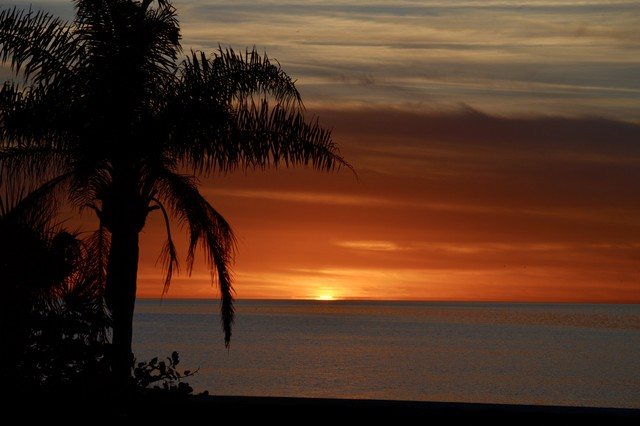
\includegraphics[height=4cm,natwidth=640,natheight=426]{images/horizon_uncropped.jpg}
			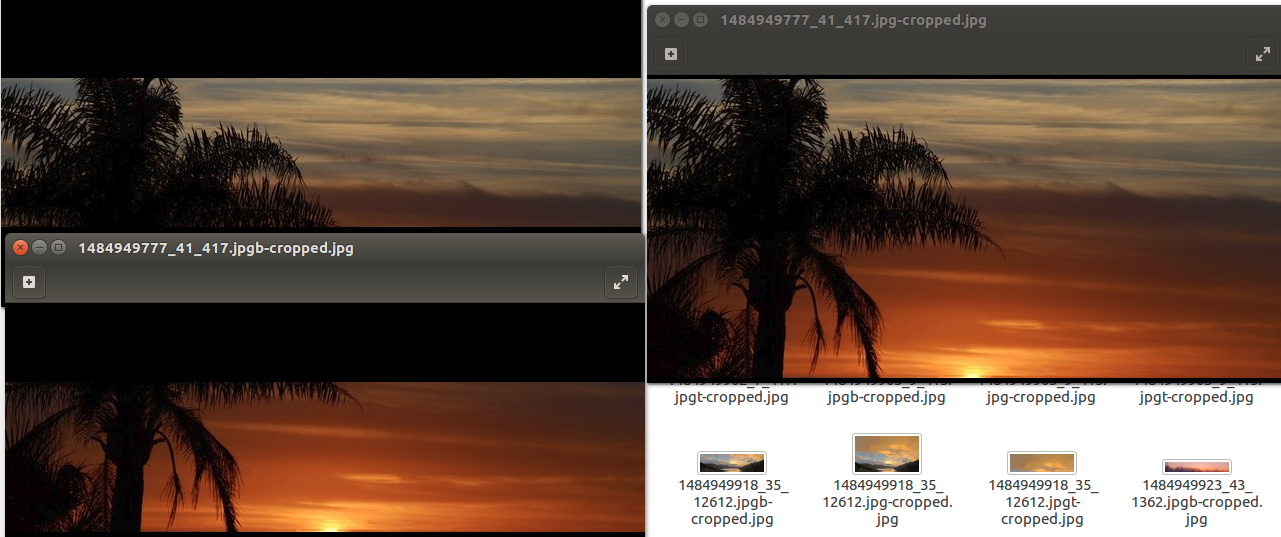
\includegraphics[height=4cm,natwidth=1281,natheight=537]{images/horizon_cropped.png}
			
\end{singlespace}
\end{document}
